%%%%%%%%%%%%%%%%%%%%%%%%%%%%%%%%%%%%%%%%%%%%%%%%%%%%%%%%%%%%%%%%%%%%%
% LaTeX Template: Praxisprojekt WS 2017
%
% Date: November 2017
%
%%%%%%%%%%%%%%%%%%%%%%%%%%%%%%%%%%%%%%%%%%%%%%%%%%%%%%%%%%%%%%%%%%%%%%

\documentclass[12pt]{article}
\usepackage[a4paper]{geometry}
\usepackage{framed}
\usepackage{footmisc}
\usepackage[myheadings]{fullpage}
\usepackage{fancyhdr}
\usepackage{lastpage}
\usepackage{graphicx, wrapfig, subcaption, setspace, booktabs}
% \usepackage{movie15}
\usepackage[T1]{fontenc}
\usepackage[font=small, labelfont=bf]{caption}
\usepackage[protrusion=true, expansion=true]{microtype}
\usepackage[ngerman]{babel}
\usepackage[ngerman]{translator}
\usepackage{sectsty}
\usepackage{url, lipsum}
\usepackage[parfill]{parskip}
\usepackage{csquotes}
\usepackage[section, acronym]{glossaries}
\usepackage{booktabs}% http://ctan.org/pkg/booktabs
\newcommand{\tabitem}{~~\llap{\textbullet}~~}
\usepackage{tabularx} % in the preamble
% \usepackage[hidelinks,pdftex,pdfpagelabels,bookmarks,hyperindex,hyperfigures]{hyperref}
% \usepackage[hidelinks]{hyperref}

% \usepackage[utf8]{inputenc}

% \bibliographystyle{numeric}

% \usepackage[style=authoryear,backref=tr"u]{biblatex}
\usepackage[sorting=none,backref=true, backend=biber]{biblatex}
\addbibresource{\jobname.bib}
% \usepackage[numbers,round]{natbib}
% \AtEveryCitekey{\clearfield{url}\clearfield{doi}\clearfield{isbn}\clearfield{issn}}


\usepackage[export]{adjustbox}
\usepackage{multicol}
\usepackage{tikz}
\usepackage{float}
\usepackage[hidelinks,pdftex,pdfpagelabels,bookmarks,hyperindex,hyperfigures]{hyperref}


\makeglossaries
\glstoctrue

%-------------------------------------------------------------------------------
% Commands
%-------------------------------------------------------------------------------
\newcommand{\HRule}[1]{\rule{\linewidth}{#1}}
\input{env}
%-------------------------------------------------------------------------------
% HEADER & FOOTER
%-------------------------------------------------------------------------------
\pagestyle{fancy}
\fancyhf{}
\setlength\headheight{15pt}
\fancyhead[L]{\newCommandName}
\fancyhead[R]{\newCommandUniversity}
\fancyfoot[R]{Seite \thepage\ von \pageref{LastPage}}

%-------------------------------------------------------------------------------
% TITLE PAGE
%-------------------------------------------------------------------------------
\begin{document}


\title{ \normalsize
		\HRule{0.5pt} \\
		\LARGE \textbf{\uppercase{\newCommandDiscipline}} \\
		\smallbreak
		\small\textbf{{\newCommandTerm}}\\
		\HRule{2pt} \\ [0.5cm]
		\normalsize \today \vspace*{10\baselineskip}}

\date{}

\author{
		\newCommandName \\
		\newCommandMatriculationNumber \\
		\newCommandUniversity \\
		\newCommandFaculty
}

% \pagenumbering{gobble}

\maketitle

\thispagestyle{empty}
\newpage
\tableofcontents
\setcounter{page}{1}

\newpage

%-------------------------------------------------------------------------------
% Section title formatting
\sectionfont{\scshape}
%-------------------------------------------------------------------------------

%-------------------------------------------------------------------------------
% 1
%-------------------------------------------------------------------------------

\section{Einleitung}
\subsection{Beschreibung des Projekts}

\subsubsection{Entwicklung einer REST-API f"ur HPC Jobs}
Cloud Computing erm"oglicht die flexible Nutzung von Computing Resources.

Durch den Einsatz von HTTP und JSON basierten Schnittstellen (REST-API's) wird es f"ur Kunden m"oglich, sehr flexibel (z.B. automatisiert) Computing Resources zu nutzen.

M"ogliche Anwendungsf"alle sind sehr vielf"altig. So kann man z.B. in einer Continous Integration Pipeline diese API nutzen. Auf diese Weise k"onnen CAE-Modelle bei jeder "Anderung durchgerechnet werden, und getestet werden, ob sie alle Anforderungen erf"ullen.

Auch die M"oglichkeit, die API in HPC Software einzubauen, die sonst auf Workstations arbeitet und anschliessend transparent Computing Resources in der Cloud nutzen kann, ist interessant. Insbesondere bei Variantensimulationen, also Simulationen, bei denen einige Parameter des Modells variiert werden, ist so eine Funktionalit"at n"utzlich. Normalerweise nutzen Ingenieure selten Variantensimulationen, da diese auf den Workstations zu aufw"andig sind.

\subsubsection{Rest-Api}

Die API soll vor allem Serverseitig umgesetzt werden. Clientseitig sollen mindestens automatisierte Integrationtests umgesetzt werden.

Der Transport/Kodierung der Daten erfolgt mittels HTTP und JSON. Die Daten sollen Transport-verschl"usselt (TLS) "ubertragen werden. Berechtigungen sollen von der API anhand geheimer Tokens gepr"uft werden.

Die API soll folgende Funktionalit"aten beinhalten:

\begin{itemize}
\item Authentifizierung / Autorisierung mittels Tokens
\item Upload der Inputfiles / Download der Outputfiles
\item Anlegen eines Jobs mittels Job Templates und Verifikation der Meta-Daten
\item "Ubergabe des Jobs an eine Queueing Engine, Abfrage des aktuellen Status und der Historie
\item Der Job soll bei der Ausf"uhrung Zugriff auf die Inputdaten bekommen und die Outputdaten anschliessend wieder in den Object-Store schreiben.
\item Ergebnisse und Metadaten bzw. Ausgabe und Fehlermeldungen des Jobs werden zum Download angeboten
\item Insbesondere soll es m"oglich sein, dass ein Job "uber die beschriebene API neue Jobs in die Queue einstellen kann. Dadurch soll der Upload von Variantensimulationen wesentlich vereinfacht und beschleunigt werden.
\end{itemize}

Es soll sp"ater viele Arten von Jobs geben und die Jobs sollen spezielle Anforderungen an die Laufzeit-Umgebung haben k"onnen (z.B. Anzahl Server und Cores pro Server). Dies soll in der Entwicklung der REST API ber"ucksichtigt werden. So soll es m"oglich sein, sich eine Liste aller m"oglichen Job-Templates und Laufzeit-Umgebungen ausgeben zu lassen.

Zugriff auf Ausgabe und Fehlermeldungen zur Laufzeit des Jobs (nicht erst nachdem er beendet ist) w"are w"unschenswert, ist aber nicht zwingend notwendig.



\subsection{Zielsetzung}

erlernen einer neuen Programmiersprache

erlernen neuer technologien

Prototyp einer rest-api (simple)

kein scaffolding oder framework

\begin{figure}[H]
  \centering
  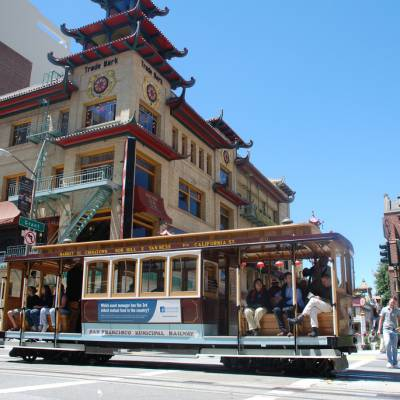
\includegraphics[width=1\textwidth]{./images/lorem.jpeg}
  \captionsetup{name=Abb.,font=footnotesize}
  \caption{Beispiel bild und beispiel cite \supercite{WinNT}}
\end{figure}

\newpage
%-------------------------------------------------------------------------------
% 2
%-------------------------------------------------------------------------------

\section{Vorgehensweise}
\subsection{Auswahl der Programmiersprache}
\subsection{Wichtige Technologien}
\subsubsection{Versionskontrolle - Git}
\subsubsection{Development und Deployment - Docker}
\subsubsection{Tools - Sequenz Diagramme - Mermaid}


\subsection{Umsetzung}
\subsection{Probleme bei der Umsetzung}

\newpage
%-------------------------------------------------------------------------------
% 3
%-------------------------------------------------------------------------------

\section{Architektur}
\subsection{Authentifizierung - Kong Api-Gateway}
\subsection{Persistenz - Mongo DB}
\subsection{Objectstore - Minio}
\subsection{Job Schedulling - Nomad}
Nomad is a single binary that schedules applications and services on Linux, Windows, and Mac. It is an open source scheduler that uses a declarative job file for scheduling virtualized, containerized, and standalone applications.


\newpage

%-------------------------------------------------------------------------------
% 4
%-------------------------------------------------------------------------------

\section{Schlusswort}
\newpage

\section{Zus"atzliche Informationen}
\subsection{Unternehmen}

CPU 24/7 ist spezialisiert auf die Vermietung und Administration
von High Performance Computing (HPC) Clustern.
Unsere Kunden sind Ingenieure, Maschinenbauer, Schiffsbauer und Autozulieferer.
Diese nutzen unsere Cluster um ihre 3D-Modelle in Physiksimulationen (Computer Aided Engineering, CAE)
zu optimieren und auf diese Weise die Entwicklungszeit von neuen Produkten zu reduzieren.

Webseite:\\
\url{https://www.cpu-24-7.com}



\subsection{Ansprechpersonen}

% \subsubsection{fachlich:}
% \texttt
\textbf{Richard Metzler M.Sc.}\\
Software Engineer Software Development

CPU 24/7 GmbH \\
August-Bebel-Stra"se 26-53\\
DE 14482 Potsdam

Telefon: +49 (0) 331 279 784 51 \\
E-Mail: r.metzler@cpu-24-7.com

% \subsubsection{organisatorisch:}
% \texttt
\textbf{Jenny Dawon M.A.}\\
Chief Administrative Officer (CAO)

CPU 24/7 GmbH\\
August-Bebel-Stra"se 26-53\\
DE 14482 Potsdam

Tel.: +49 (0) 331 279 784 44\\
E-Mail: j.dawon@cpu-24-7.com

\subsection{Ressourcen}
\textbf{Git-Repository als Versionskontrolle:}\\
\url{https://github.com/MatthiasHertel/ws17_pp}

\textbf{Webseite zur Dokumentation:}\\
\url{https://www.ws17-pp.mhertel.de}



%-------------------------------------------------------------------------------
% Literatur - Glossar - Akronyme
%-------------------------------------------------------------------------------
% \renewcommand\glossarytitle{}
\clearpage
\setlength\bibitemsep{10pt}
\printbibliography[heading=bibintoc, title=Quellenverzeichnis]
\newpage
\phantomsection
\addcontentsline{toc}{section}{Abbildungsverzeichnis}
\listoffigures
\newpage

% \printglossary[type=\acronymtype, title=Abk"urzungsverzeichnis]
% \newpage
%
% \printglossary[type=main,title=Glossarverzeichnis]
% \newpage



%-------------------------------------------------------------------------------
% ENDE
%-------------------------------------------------------------------------------

\end{document}
